\documentclass[12pt, a4paper]{article}
\usepackage[margin=2.0cm]{geometry}
\usepackage{stmaryrd}
\usepackage{amsmath}
\usepackage{amssymb}
\usepackage{enumerate}
\usepackage{bbold}
\usepackage{dsfont}
\usepackage{wrapfig}
\usepackage{algorithm2e}
\usepackage{changepage}
\usepackage{undertilde}
\usepackage{hyperref}
\hypersetup{pdftex,colorlinks=true,allcolors=blue}
\usepackage{hypcap}
\usepackage{multicol}
\usepackage{float}
\usepackage{tikz}
\usepackage{qtree}
\usepackage[amsmath,hyperref]{ntheorem}
\usepackage{framed}
\usepackage{booktabs}
\usepackage{needspace}
\usepackage{color}
\usepackage{listings}
\usepackage{xifthen}
\usepackage{graphicx}
\usepackage{caption}
\usepackage{subcaption}

\setlength{\parskip}{\baselineskip}

\title{Computational Neuroscience Coursework 2}
\author{Dylan Cope (dc14470)}
\date{}

\renewcommand\vec[1]{\mathbf{#1}}
\newcommand\uvec[1]{\hat{\mathbf{#1}}}

\begin{document}

\nocite{*}
\bibliographystyle{plain}

\maketitle

\begin{figure}[H]
  \centering
  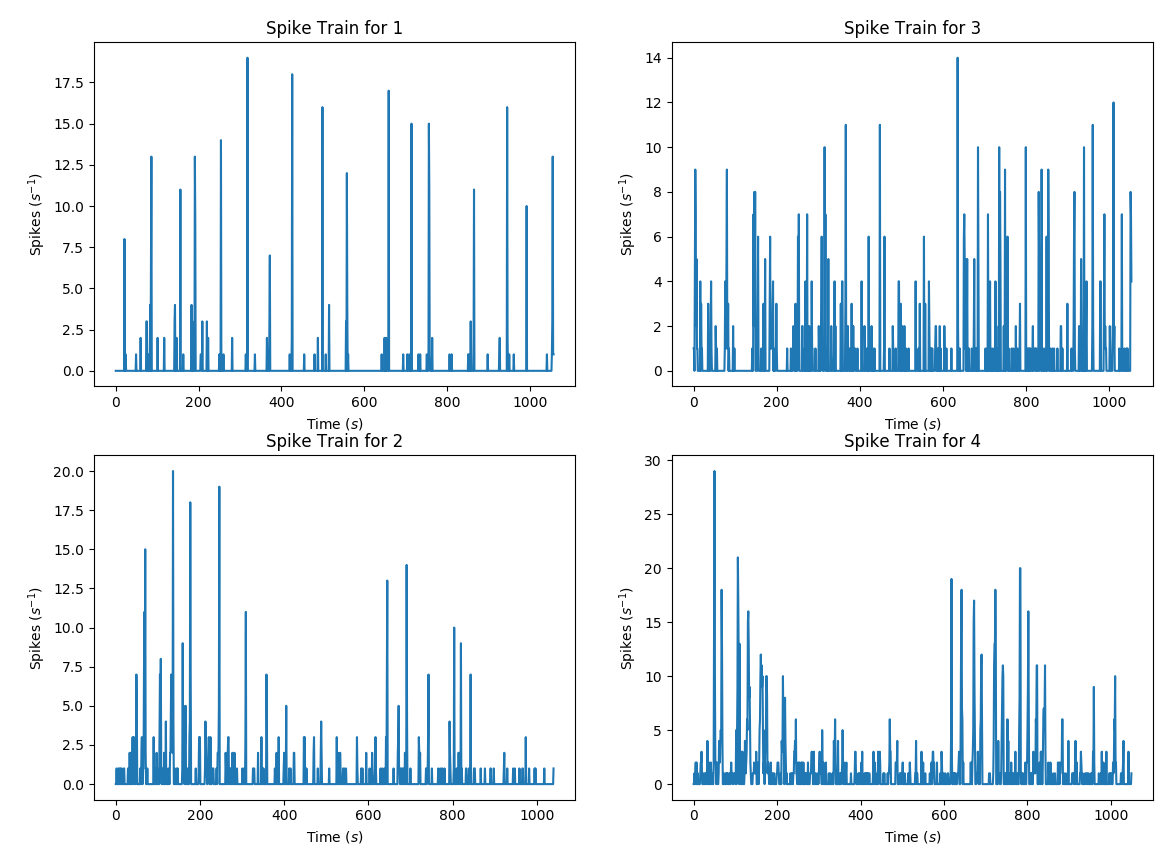
\includegraphics[width=\linewidth]{../figures/spike_trains}
  \caption{Spike trains for the four neurons} \label{spike_trains}
\end{figure}


\begin{figure}[H]
  \centering
  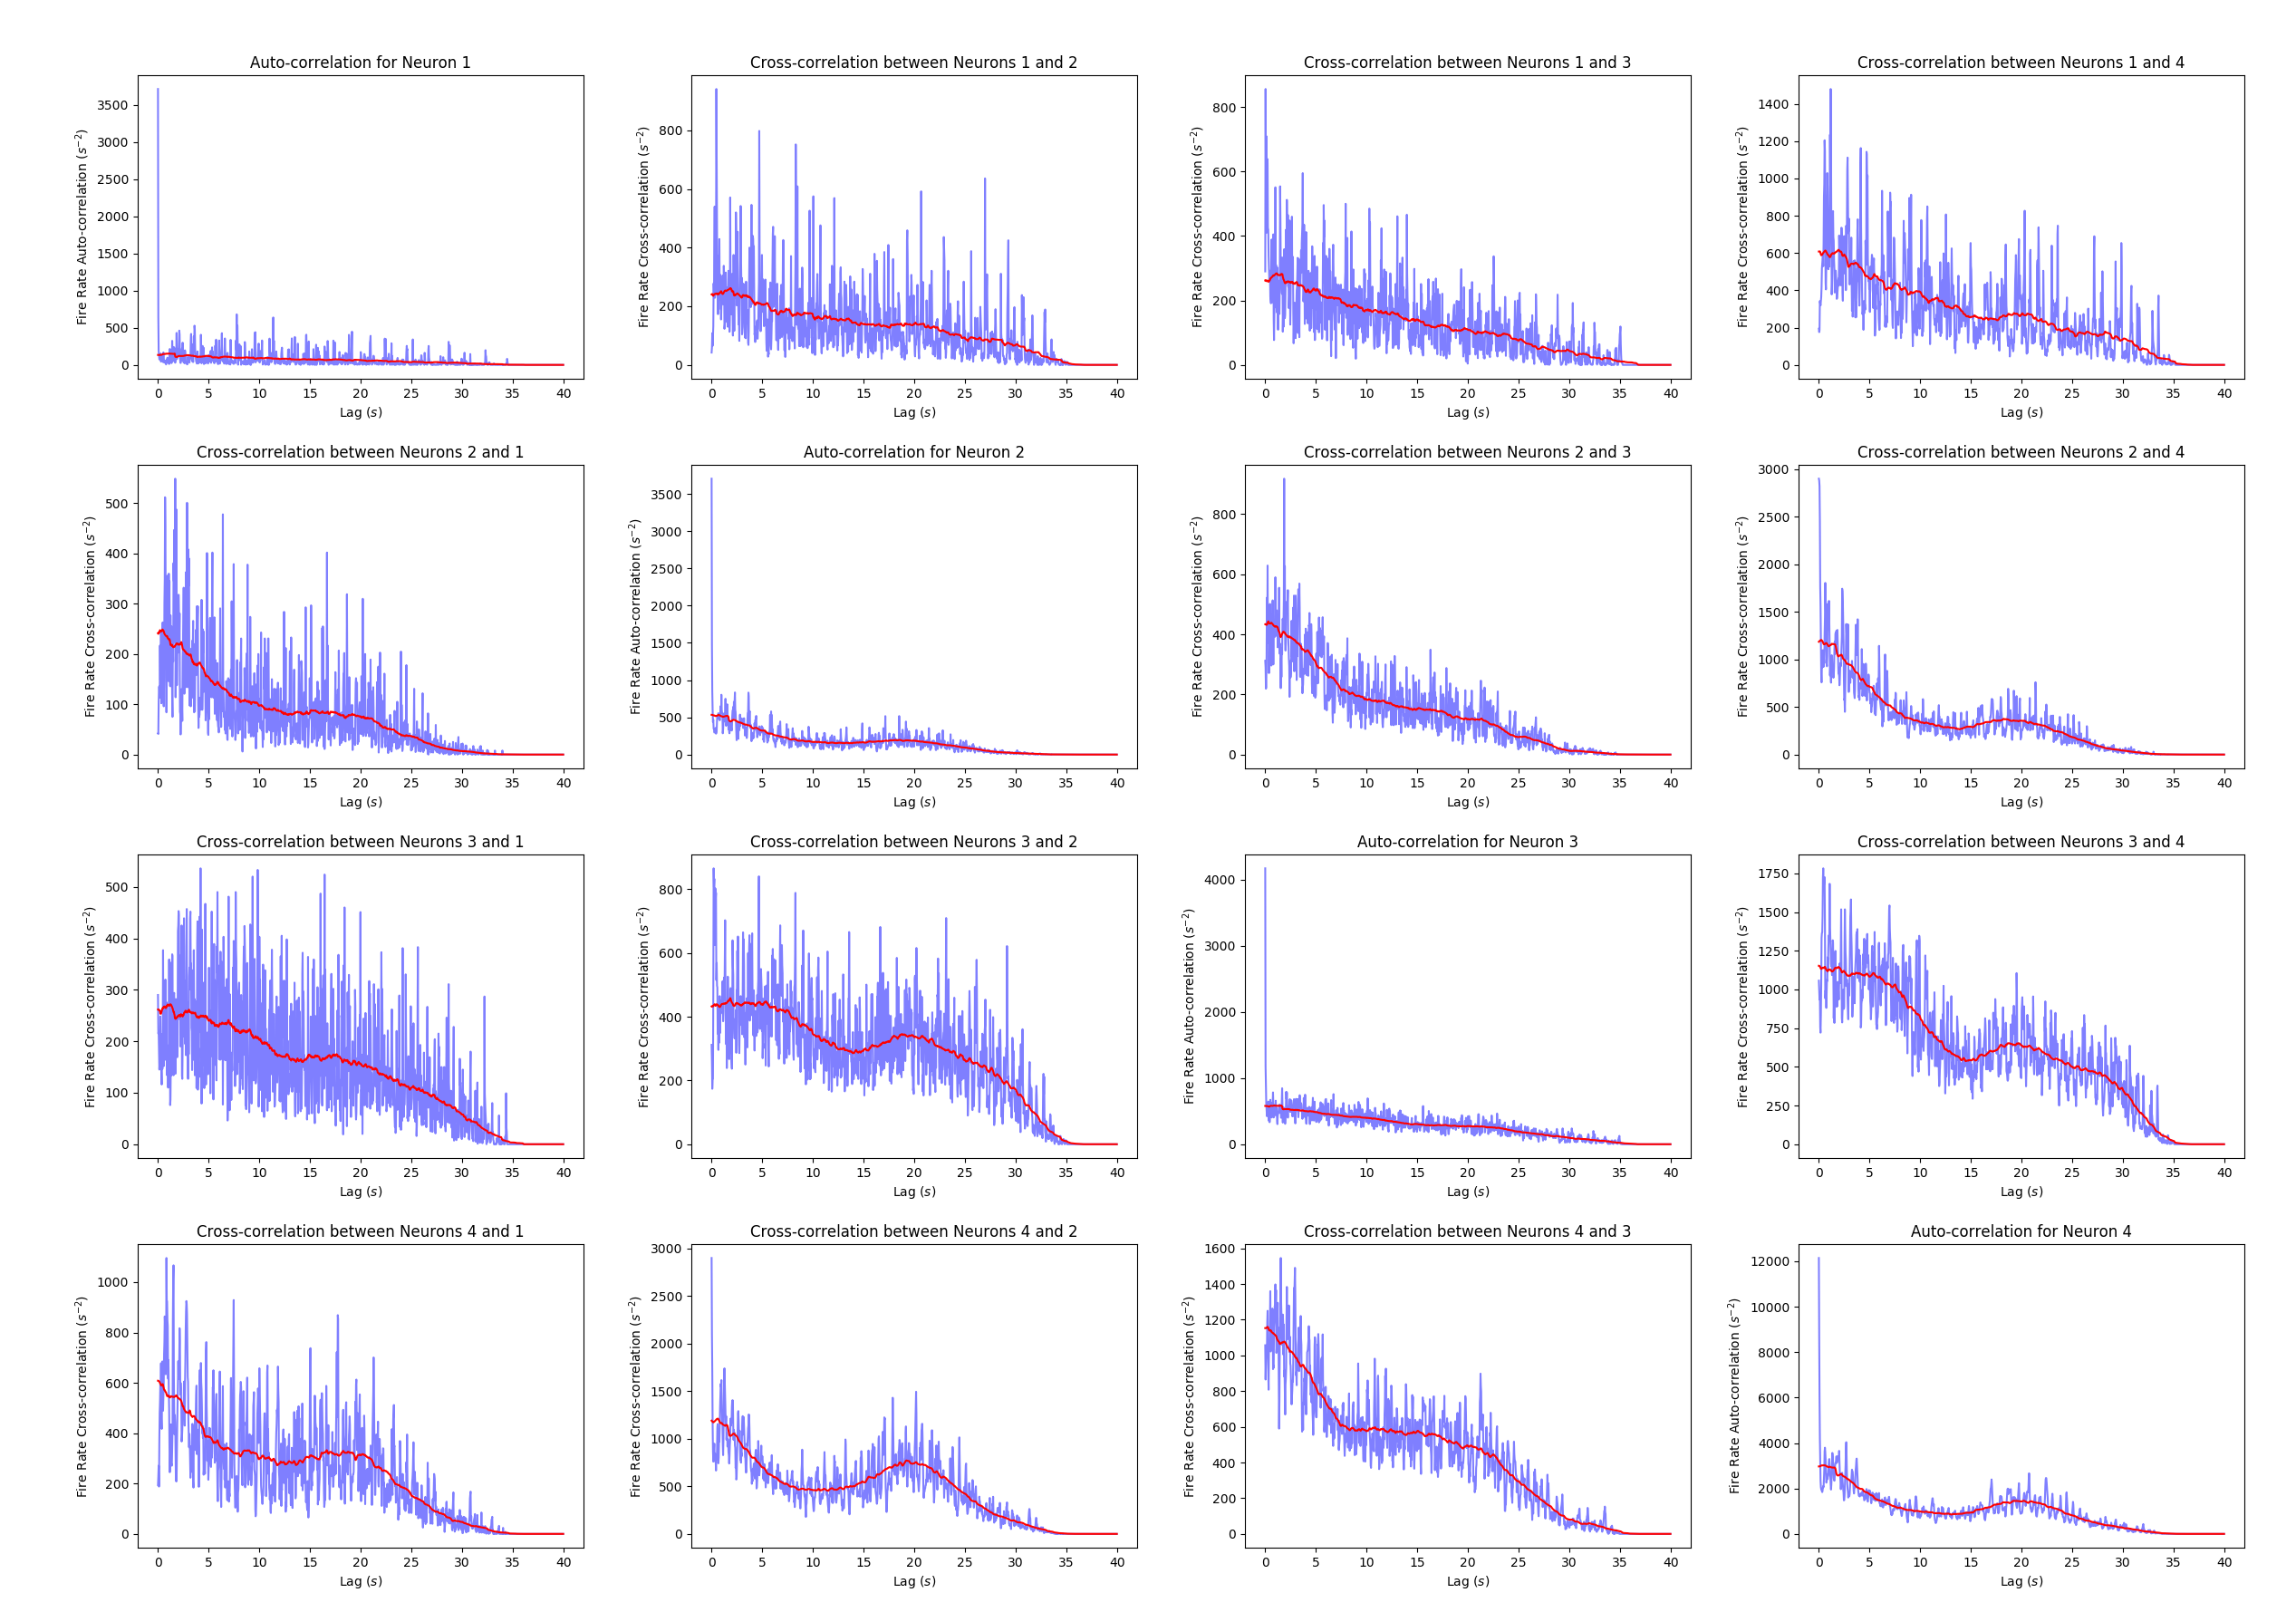
\includegraphics[width=\linewidth]{../figures/correlations}
  \caption{Spike trains cross-correlations} \label{correlations}
\end{figure}


\begin{figure}[H]
  \centering
  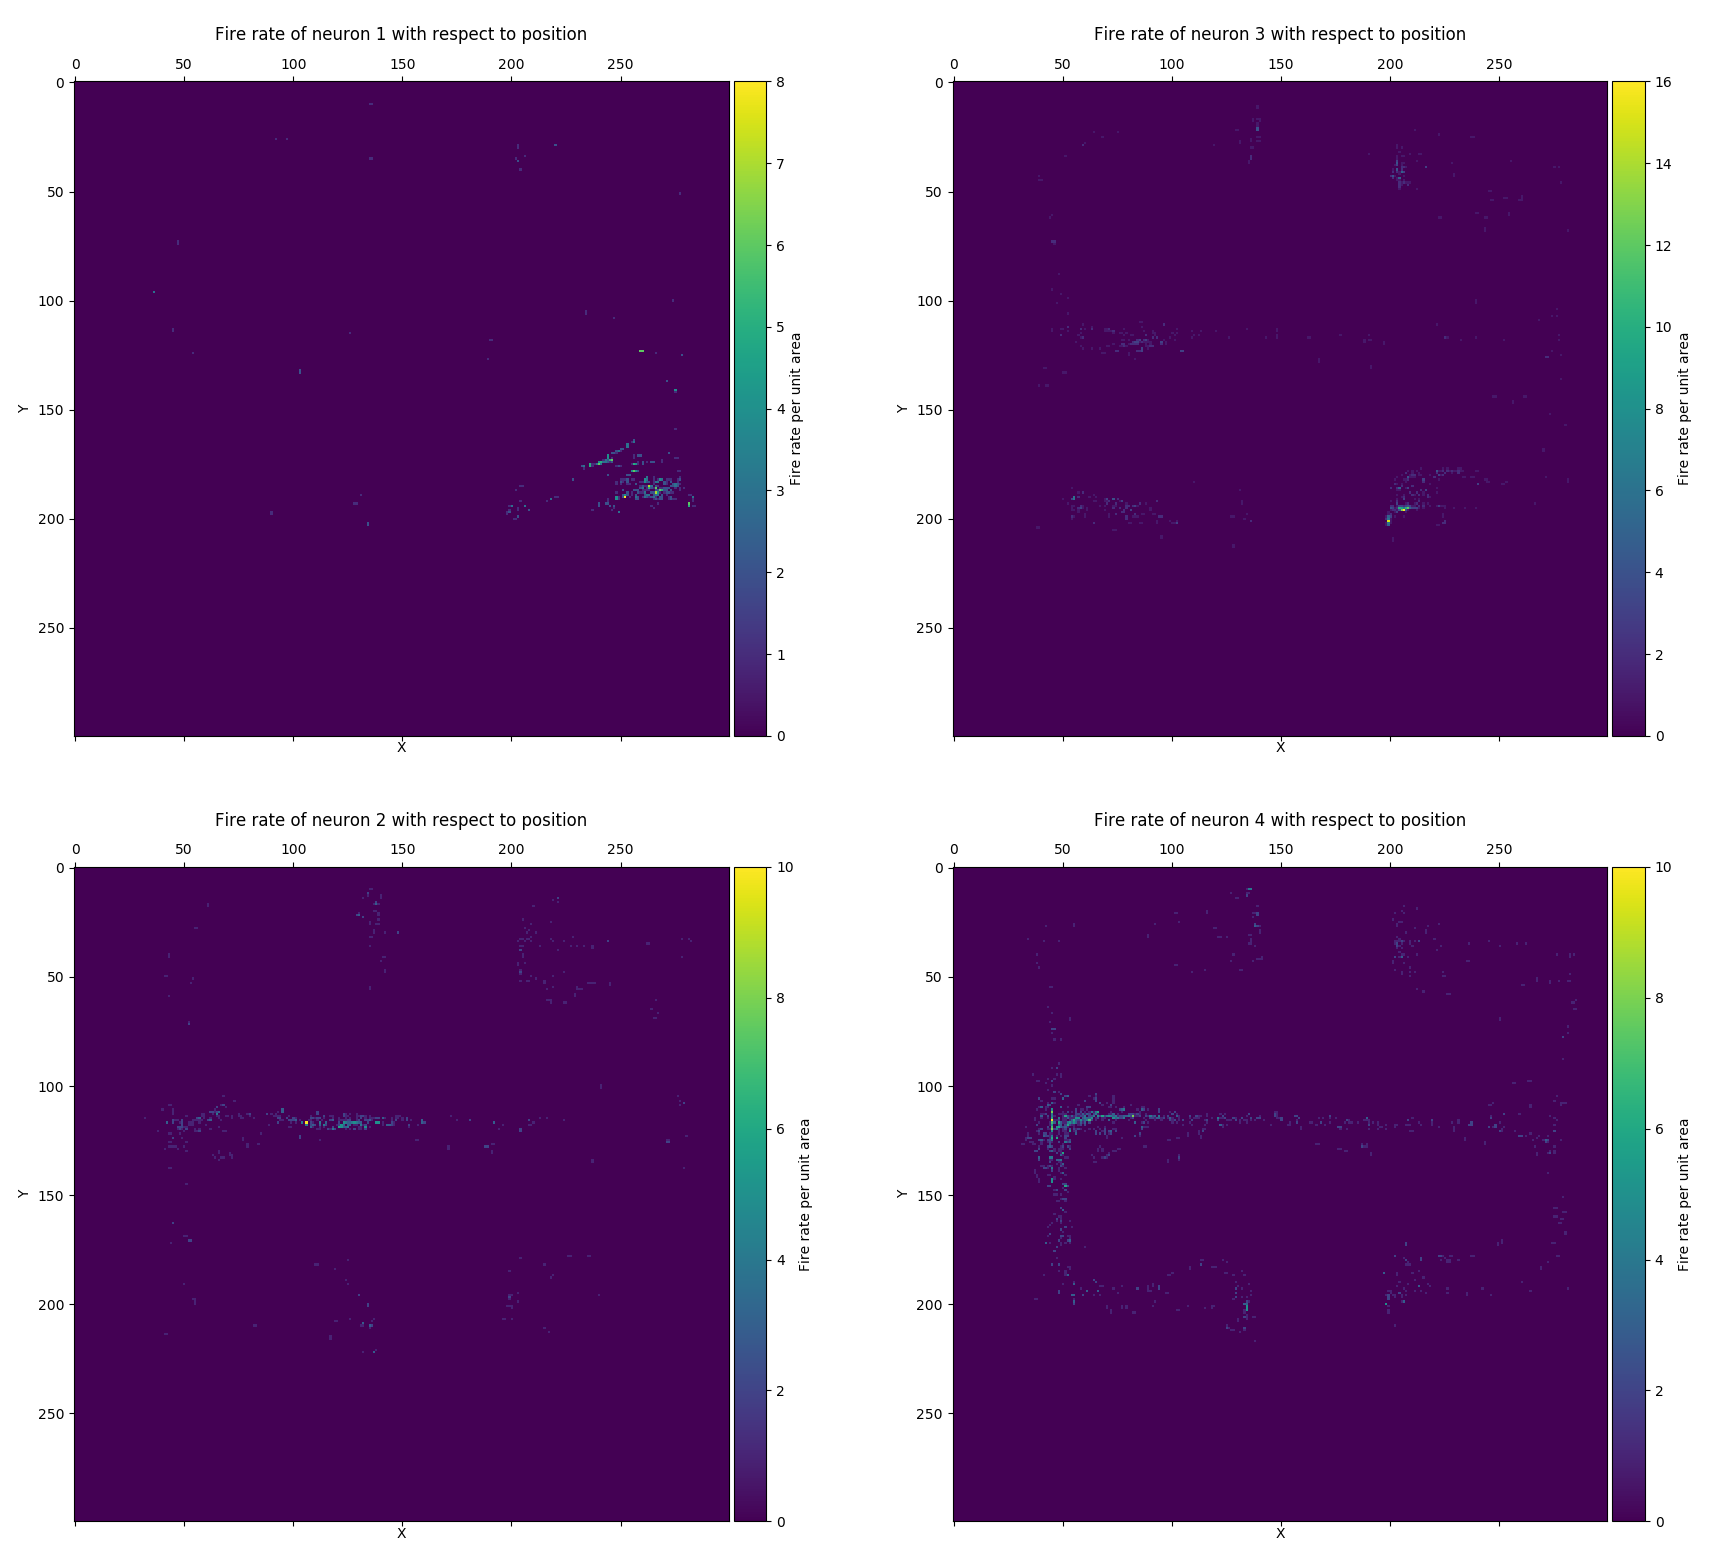
\includegraphics[width=\linewidth]{../figures/spatial_fire_rates}
  \caption{Fire rate per unit area for each neuron} \label{spatial_fire_rates}
\end{figure}

\bibliography{dc14770}
\bibdata

\end{document}
